\subsection{Menu} \label{subsec:menu}
The menu is a lot more complicated than the HUD which is described in \autoref{sec:hud}.
Because of that, we decided to create a framework for creating menus.
This framework was heavily inspired by Flutter \cite{flutter}.
It uses the same concepts and terminology.
The overall idea is that everything is a widget.
A widget is a class that has a \texttt{Render} method as well as a \texttt{GetSize} method.
The \texttt{Render} method takes a context that includes information about the position and size on the screen that the widget can render to.
Some widgets also have children so the overall structure of the menu is a tree of widgets.

An example of a widget is shown in \autoref{fig:example_widget}.
This widget renders the main menu of the game.
The rendering logic of this widget can be seen in \autoref{fig:widget_logic}.
The idea is as follows.
The root widget calls the render method of its child which is the \texttt{Background} widget.
The \texttt{Background} widget renders a background color.
Then the \texttt{Background} widget calls the render method of its child which is the \texttt{Column} widget.
This widget renders its children in a column but to do that it first needs to know the size of each of its children.
Based on that information it will call a render method of each child with the appropriate context.
Each child asks its children for their size recursively until it reaches a leaf widget.
The process stops at the leaf and the render method is called on the children of the column widget.

This is a simplified version of the rendering logic as each widget has multiple options and rules that change how it or its children are rendered.
For example, the \texttt{Column} widget has a \texttt{alignment} property which changes how the children are aligned.
The \texttt{Button} widget in the \autoref{fig:widget_logic} itself is a tree of widgets.

This approach to rendering the menu is very flexible and allows for a lot of customization.
It improves on the method used to render the HUD described in \autoref{sec:hud}.
This approach is not common in game development.
Usually, menus are created by putting elements on the screen at specific positions.
In this part, we believe that our approach is better than the traditional one and improves on approaches used in for example Godot \cite{Godot-Menu}.
\todo{Is this citation enough for this claim?}

\begin{figure}[H]
    \centering
    \begin{subfigure}{0.45\textwidth}
        \centering
        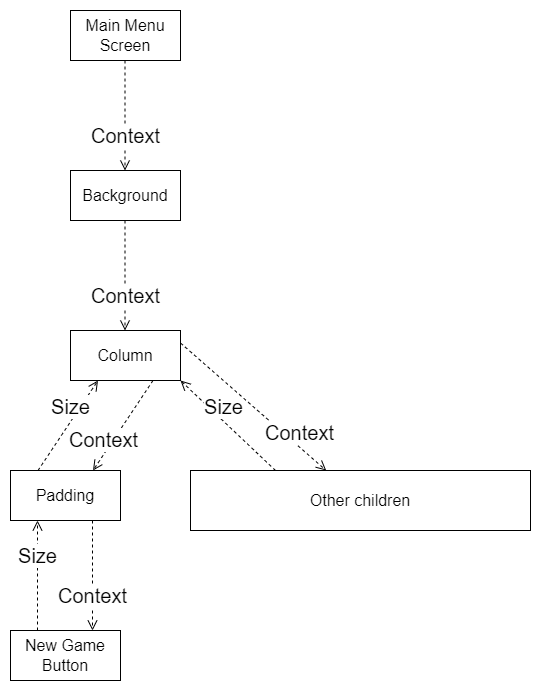
\includegraphics[width=0.8\textwidth]{chapters/system_architecture/sections/two_dimensional_graphics/resources/widget_logic.drawio.png}
        \caption{Widget rendering logic.}
        \label{fig:widget_logic}
    \end{subfigure}
    \hfill
    \begin{subfigure}{0.45\textwidth}
        \centering
        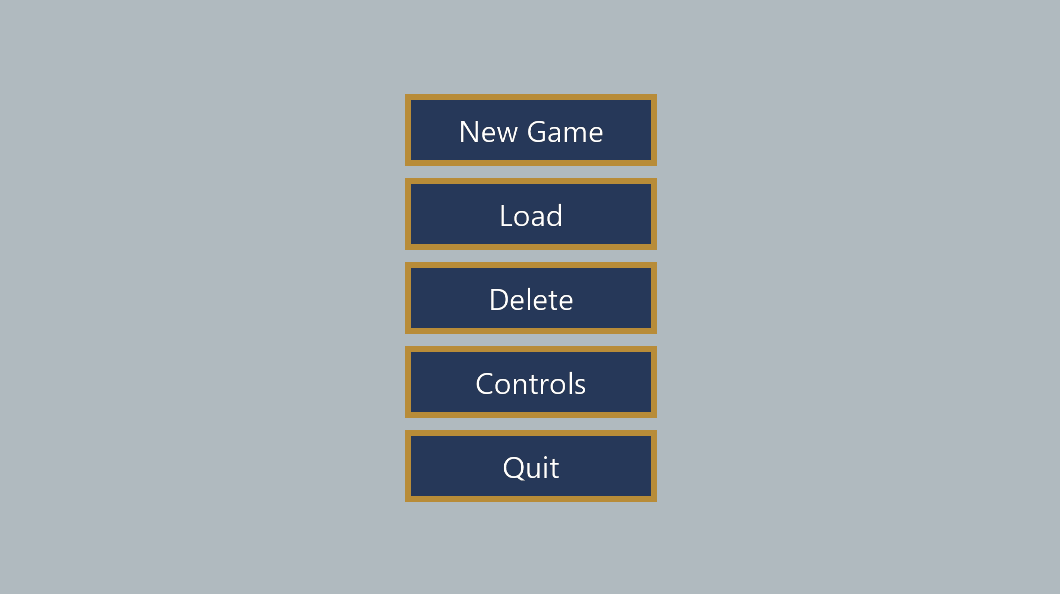
\includegraphics[width=0.8\textwidth]{chapters/system_architecture/sections/two_dimensional_graphics/resources/main-menu.png}
        \caption{Main menu.}
        \label{fig:example_widget}
    \end{subfigure}

    \caption{Example widget.}
\end{figure}